\documentclass[12pt,a4paper]{article}

\usepackage{indentfirst}
\usepackage{blindtext}
\usepackage[utf8]{inputenc}
\usepackage{graphicx}
\usepackage{booktabs}

 
\title{MCSED: Matching Observations to Model SEDs}
\author{Hunter Brooks}
\date{\today}
 
\begin{document}
\maketitle

\section*{}
MCSED is the easy to use, all inclusive tool for matching observational data to model Spectral Energy Distributions (SEDs) thereby retrieving the physical parameters of the models such as stellar mass, metallically, dust mass.  The code uses Charlie Conroy's Flexible Stellar Population Synthesis (FSPS) Fortran 90 code to generate model SEDs and a Markov Chain Monte Carlo Python simulator called emcee to explore the likelihood of matches to input data.  For ease of use, Python FSPS is used to wrap FSPS, requiring the user to only modify simple Python scripts in order to customize the package for any specific need.  

This guide is a very rough overview of how to use MCSED and was written for the Penn State Dep't of Astronomy and Astrophysics.  

Note: [underscore] in this guide means the actual symbol.  
\newpage
 
 

\section{Overview}

This software package seeks to be the simple, single download required to match observational data to model SEDs.  It's main use is to match observational data over many bands to model SEDs created using know parameters.  Once a match is obtained, one can infer the observed object has the model parameter values used to create the model SED along with the physical characteristics predicted by the model.  Also one can observe the relationship of the likelihood of match between these parameters.  

Of course, the accuracy of the result is dependent on the way Stellar Population Synthesis is conducted. Conroy's FSPS was chosen for its flexibility and speed.  MCSED uses a python front end, called python-fsps, to interact with FSPS.   Python-FSPS was developed by Dan Foreman Macky.  

Because FSPS SEDs require model parameters as inputs, when matching observational data to models, a multidimensional parameter space is explored.  To explore the parameter space, a software package called ``emcee" is used.  Emcee is a Markov Chain Monte Carlo Metropolis Hastings simulator.  Walkers venture into a parameter space, conducting a random walk during which the desirability of parameter space location is determined by a $\chi^2$ relationship between the observational filter data and the computed average flux in the appropriate bands for the model.  The emcee code requires its own inputs (characteristics of the walkers) that relate to the accuracy of run time results.  

This software package contains all the code to create a parameter space, estimate emcee parameters, and run a emcee random walk.  The user simply needs to define which FSPS parameters they intend to explore.  This package was created initially to investigate the Draine \& Li 2007 dust emission model, a model FSPS is capable of producing.  I strongly recommend the user understand the basics of FSPS and emcee.  Also note that additional helpful information can be found in the comments within each script.

One of the most useful functions of MCSED is the built in self test mechanism.  Once a user decided which FSPS parameters to explore and in which astronomical bands to do so, MCSED can pick random values for these parameters and create a SED using FSPS.  Random noise (gaussian, $\mu = 1.0, \sigma = 0.10$) is then added to the SED.  This emission SED is then redshifted and converted to filter measurements, as one would observe.  At this point, MCSED estimated what a galaxy with known parameter values will look like in the filters in question.  These psuedo-observations can then be fed into MCSED (and have the random walk process done on them) and hopefully the software recovers the random parameter values chosen.  This technique is good for testing your technique and finding a healthy balance between run time and accuracy.  

Please also note that MCSED can search the parameter space via two methods: interpolation of a premade parameter space, or direct SED calculation given parameter values.  For my projects, direct calculation was necesary because the SEDs in the premade parameter space results in very bumpy chi squared values.  MCSED can work in the premade by modified a value in main.py, if you'd like more information about this email hunterbrooks16@gmail.com.  The mode is set by the vHouse.walker[underscore]SED[underscore]type variable in main.py.


\section{Table of Contents}

In this manual, I explain how to install MCSED, use the code, and detail the scripts and functions found within the package. In \S 3 I describe how to install MCSED and its components; the software is designed to be easy to install.  In \S 4 I outline the environment of MCSED and the function of each file so the reader can get his bearing in the system.  This leads into \S 5 which is a discussion of how MCSED works and its available parameters.  The average user will likely need to customize the software and this section seeks to make this process as easy as possible.  In \S 6 I explain how to import your own data into MCSED







\section{Installation}

\textbf{This section may be out of date.}  Installation of MCSED is simple, but nontraditional.  For MCSED to run, FSPS needs to be installed and compiled, and python-FSPS and emcee need to be installed.  Bellow are the combined installation instructions for the relevant software packages.   

\begin{enumerate}
\item Download FSPS by typing SVN -r 143 GET in a terminal window.  Note that we got FSPS svn version 143.  This is necessary for the current version of python-fsps.
\item Set a home variable of the name SPSHOME to the location of the FSPS folder.
\item in SPSHOME/src/compsp.f90 change line 685[?] to read: 1e5.  This avoids errors, though to be honest we're not entirely sure exactly why this is necessary.  My hunch is that there is a bug in python-fsps.  
\item Compile the code in SPSHOME/src/ using make clean and make.  At this point its recommended that you test that FSPS has install correctly by typing "./simple.exe".
\item Install Python version 2.7.9 via the website:.  An alternative for this step can be to install a python studio such as anaconda.  Most come with Numpy and Scipy.
\item Install Numpy.  
\item Install Scipy.
\item Using pip, install python-fsps.
\item Install emcee
\item Run install test script. [This hasn't been written yet.]

\end{enumerate}


Make sure Numpy, Scipy, cPickle, FSPS, python-fsps are all installed correctly. Compile the FSPS  code.  Note that python-fsps works on a slightly older version of FSPS so make sure you follow the installation instructions on the website below.  Also for displaying data matplotlib might be useful.  

Locations of the packages: 


\begin{centering}

Numpy: http://www.numpy.org/ 

Scipy: http://www.scipy.org/

FSPS: http://people.ucsc.edu/~conroy/FSPS.html

python-fsps: http://dan.iel.fm/python-fsps/current/

\end{centering}






\section{The Environment}

\begin{figure}
\begin{centering}
	%top of pendulum with point mass
	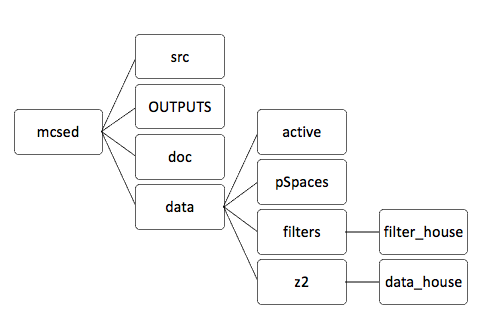
\includegraphics[width=1.0\textwidth]{/Users/hunterbrooks/astronomy/dust/doc/mcsed_ftree.png}
	\caption{File tree of MCSED.}
	\end{centering}
\end{figure}

Figure 1 shows the folder hierarchy of MCSED.  Each folder and its components are outline below



\begin{enumerate}
\item src - holds all off the code written for MCSED.  All script edits are done in this folder.
\item OUTPUTS - holds the outputs of your software in .npz format.
\item doc - any documents included in your MCSED release
\item data - folder that contains all the input data 
\begin{enumerate}
\item active - MCSED needs a few inputs to run, they're kept in this folder.  anything with the prefix "super" holds all the observational information (galaxy redshifts, filter measurements, etc). anything with the prefix "filter" relates to the filter wavelengths (angstroms) or names.  
\item pSpaces - holds premade parameter spaces, only used when in vHouse.walker[underscore]SED[underscore]type == 'Interp' in main.py
\item filters - separates filter files from everything else. contains the list of filter names and central wavelengths.
\begin{enumerate}
\item filter house - actually holds the filter curves, normalized to 1, in angstroms.
\end{enumerate}
\item z2 - i created this folder to house all the information about my catalog of redshift = 2 galaxies.  really, this doesnt need to exist.  all that is necesary is the ``super"XXX files in active, but in this folder i keep my catalogs and the scripts to take the important galaxy data from the catalogs and make a usable set of ``super"XXX files.
\begin{enumerate}
\item data house - where i keep catalogs of raw observations.
\end{enumerate}
\end{enumerate}
\end{enumerate}






\section{How MCSED Works}

\begin{enumerate}
\item obtain scientific observations of galaxies in many filters
\item obtain redshift measurements for those galaxies
\item obtain filter curves for each filter you'd like to use. note: not every object must have an observation in every filter.
\item write custom code that interfaces with your catalog to create superErrors.dat, superFluxes.dat, superIndexes.dat, superInfo.dat, and superRedshift.dat.  Follow the format given in the example superXXX.dat files.  Reference main.py because main.py reads the superXXX.dat files.  
\item create filter[underscore]lambdas.dat and filter[underscore]names.dat containing central filter wavelengths and names.  Put these in /data/active.
\item Recommended: Create a few test objects via the make[underscore]test.py script.  This script will make a set of superXXX.dat for some psuedo-objects.  Then, run MCSED on these pseudo-objects.  Confirm that the orgional parameters are recovered by analysisng the .npz file created in /OUTPUTS.  You might want to use my interpret[underscore]results.py for help doing this.  Also, reference main.py to see how the .npz files are created. 
\item Modify the emcee parameters (number of walkers, number of steps taken, number of steps in the burn in chain) to fine tune accuracy of results.  Experiment with this.  Read about emcee, they have at least one good paper out on the software.  Check the acceptance fraction.
\item With the superXXX.dat files corresponding to your non-test galaxies in /data/active, run MCSED via main.py. 
\item Note: At the current configuration MCSED supports parallelization.  Simply set nScriptsRunning in main.py to a number greater than 1.  You also need to copy main.py that many times (naming the files 01main.py, 02main.py, ...etc).  You can then run the numbered main.py's in parallel. 
\end{enumerate}



If you really would like to modify MCSED, email hunterbrooks16@gmail.com with questions.  However, MCSED works as is!








\section{Importing Data}

Importing data is done by simply writing a script to create a set of superXXX.dat files.  Reference my superXXX.dat files and main.py (the script that reads them). 




\end{document}
